\section{Concept Number Upper Bound Prediction}\label{sec:upper-bound}
In sequence generation, there are two approaches on how to generate the correct number of elements.
The first option is to interrupt the generation based on a value generated at each step by the model, \eg, a stop value equal to 1 when generating the last element.
The alternative is to determine the number of elements beforehand and generate exactly this number of elements.
To generate the correct number of intents, we decided to use the second option, given the performance of the concept number predictor learned with BoA. Indeed, the number of intents is equal to the number of concepts in the lattice.

In our case, we have a margin of error in the predicted number of concepts $\hat{|I|}$.
Indeed, the generative model (phase 3 of the approach) will be able to compensate by filling the excess space with empty intents if $\hat{|I|}$ is higher than the actual number of concepts.
However, if $\hat{|I|}$ is too low, the generative model will not have enough space to generate the intents.
In short, we need an upper bound of the number of concept rather than the number of concept itself.
The additional freedom makes it easier to design a model fitting our needs.

We could use a theoretical upper bound, but those are rather large and increase exponentially with the size of the data (see \cref{sec:boa-metric-perf}).
Instead, we train a MLP to predict an upper bound of the concept number, from the prediction of the model learned with BoA and an average-pooling of the attribute embeddings. We train this model using an adapted MSE described in \cref{equ:upper-bound-loss}, with $p$ the target and $q$ the predicted number of concepts.
This new loss function first shifts the prediction target 10\% higher than the actual concept number, and penalizes predictions under the target by multiplying the squared error by 100 (an arbitrary number which provided good results).

We show in \cref{fig:concept-upper-bound} the upper bounds predicted on the validation set.
Of the 1000 samples tested, less than 1.2\% of the predictions are under the actual concept number.
The remaining prediction are close to the actual numbers, in average around 125\% of the true concept number.

\begin{figure}
    \centering
    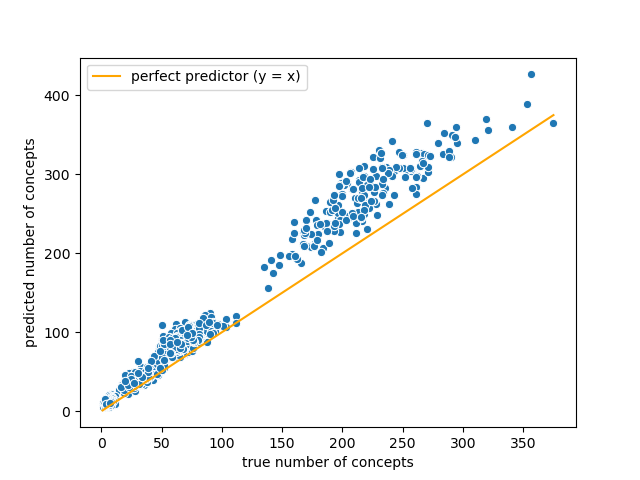
\includegraphics[keepaspectratio, width=.9\textwidth]{Figures/Ch3/concept_upper_bound.png}
    \caption{Upper bounds predicted by the model on all the samples of the evaluation set.}
    \label{fig:concept-upper-bound}
\end{figure}

\begin{equation}
    \begin{split}
        ShiftedError(p, q) &= q - (p \times 1.1)\\
        UpperBoundError(p, q) &= ShiftedError(p, q)^2 \;\text{~~if } ShiftedError(p, q) > 0\\
        &= 100 \times ShiftedError(p, q)^2 \;\text{~~otherwise}
        \label{equ:upper-bound-loss}
    \end{split}
\end{equation}